% \input{\pSections sec-geometry}

\section{Geometry of Kepler's Law}
\label{sec:geo}

\begin{figure}[htbp] %  figure placement: here, top, bottom, or page
\centering
\begin{center}
   \includegraphics[ width = 3.75in ]{\pLocalGraphics vallado-anomaly} 
   \caption{Vallado's figure 2-2 showing $E$ and $\nu$.}
\end{center}
   \label{fig:anomaly-vallado}
\end{figure}

\begin{figure}[htbp] %  figure placement: here, top, bottom, or page
\begin{center}
   \includegraphics[ width = 3.5in ]{\pLocalGraphics Bate-etal-anomaly} 
   \caption{Figure 4-4 in Bate \emph{et al.}  showing $E$ and $\nu$.}
\end{center}
   \label{fig:anomaly-bate}
\end{figure}

\begin{figure}[htbp] %  figure placement: here, top, bottom, or page
   \centering
   \includegraphics[ width = 4in ]{\pLocalGraphics moulton-anomaly} 
   \caption{Moulton's figure 28 showing $E$ and $\nu$.}
   \label{fig:anomaly-mouton}
\end{figure}

\begin{figure}[htbp] %  figure placement: here, top, bottom, or page
\centering
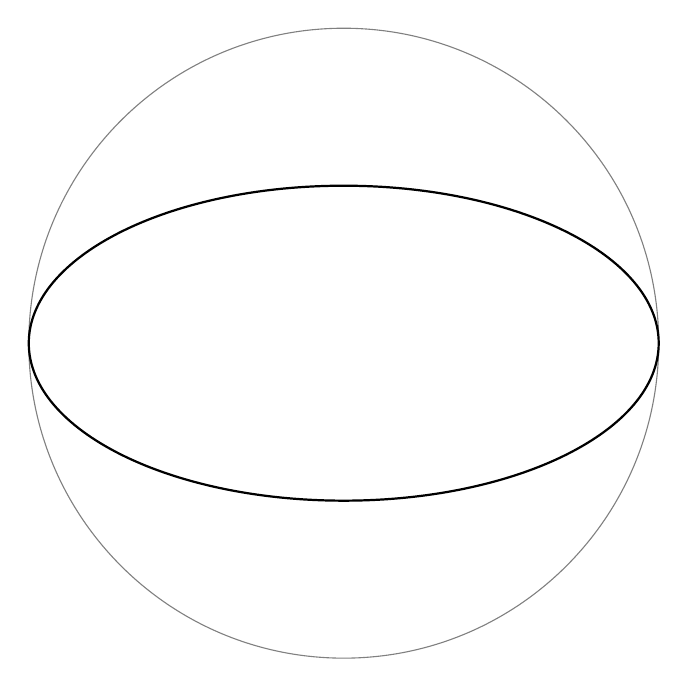
\begin{tikzpicture}
	\draw[gray] (0,0) circle (4cm);
	\draw[thick] (0,0) ellipse (4cm and 2cm);
\end{tikzpicture}
\caption{Geometry}
\label{fig:ellipse-circle}
\end{figure}

%\begin{table}[htp]
%%\caption{default}
%\begin{center}
%\begin{tabular}{ccc}
%	%
%   \includegraphics[ width=2in ]{\pLocalGraphics vallado-anomaly} 
%	%
%   \includegraphics[ width=2in ]{\pLocalGraphics vallado-anomaly} 
%	%
%   \includegraphics[ width=2in ]{\pLocalGraphics vallado-anomaly} 
%	%
%\end{tabular}
%\end{center}
%\label{default}
%\end{table}%

Disagreement with this YouTuber \href{https://www.youtube.com/watch?v=cf9Jh44kL20}{True Anomaly vs. Mean Anomaly}

\endinput  %  ==  ==  ==  ==  ==  ==  ==  ==  ==
